%
% Uvod
%

\chapter{Úvod}

Každý linuxový server alebo osobný počítač môže slúžiť na niečo iné. Preto je
veľmi náročné vytvoriť linuxovú distribúciu, ktorá by pokrývala požiadavky
každého a~bola optimalizovaná pre všetky operácie. Preto je potrebné systém
nastaviť tak, aby presne vyhovoval naším potrebám a~získali sme maximálny výkon
pre naše potreby. Kedže sa jedná a~množstvo druhov nastavení, vznikol balíček
\emph{tuned}\cite{tunedHomepage}, ktorý ich zahrňuje.

Cieľom tejto práce je priblížiť \emph{tuned}, zhrnúť jeho hlavné funkcie,
popísať profily a~na záver implementovať sadu testov pre I/O operácie nad
najpoužívanejšími súborovými systémami a~diskovými zariadeniami. Na záver budú
testy spustené a~výsledky vyhodnotené.

%
% Popis komponenty
%

\chapter{Popis komponenty tuned}

Balíček \emph{tuned} je primárne napísaný pre linuxovú distribúciu
Fedora\cite{fedoraHomepage} a~Red Hat Enterprise Linux. Démon \emph{tuned} neustále
beží, skenuje systém a~upravuje nastavenia podľa potreby. Napríklad najväčšia
záťaž na disk je pri štarte systému alebo pri ukladaní dát na disk (napríklad
filmov). Inak je disk skoro nečinný. \emph{tuned} dokáže optimalizovať zápis práve v
tej dobe, keď je to potreba. Rovnako je to aj pri sieťových operáciach.

Niektoré profily zamedzujú aj prepínaniu Cx stavov \footnote{Cx sú stavy, v
ktorých sa môže vyskytovať procesor, typicky firmy Intel. Tieto stavy sa volajú
Spiacie stavy (ang. Sleep states) \cite{sleepStates}. Spiace stavy procesoru
slúžia na šetrenie energie.}.

Súčasťou \emph{tuned} je aj program \emph{tuned-adm}, ktorý nám dovoľuje
prepínať medzi profilmi. Každý z~profilov slúži na iné zameranie a~napriamo
podľa toho upravuje systém, čím dosahujeme ešte lepšie výsledky.

%
% Historia tuned
%

\subsection{História \emph{tuned}}
\label{sec:historiaTuned}

%TODO: Skontrolovat rok
Komponenta \emph{tuned} je vyvýjaná od roku 2008. Prvými autormi boli
\emph{Philip Knirsh} a~\emph{Thomas WoVerner}. Dnes sú najväčšími
prispievatelia \emph{Ján Včelák}, \emph{Jaroslav Škarvada} a~\emph{Ján Kaluža}.
Dnes je \emph{tuned} vo verzii \emph{2}. Medzi verziou \emph{1} a~\emph{2} je
veľký rozdiel, pretože bol celý kód od základov prepísaný. Jedna z~najväčších
zmien je v~používaní \emph{D-BUS} \footnote{Systém pre jednoduché zasielanie
správ a~komunikáciu medzi aplikáciami}. Ďalšia zmena je v~profiloch. Niektoré
profily boli zmenené alebo odobraté. Pre zachovanie spätnej kompatibility
vznikol preto balík \emph{tuned-profiles-compat}, ktorý obsahuje všetky profily
z verzie \emph{tuned 1}.

%
% Profily tuned
%

\section{Profily}

Profily su hlavne zamerané na CPU, disky, sieť a~FSB \footnote{Front-Side Bus -
datová zbernica, ktorá zaisťuje komunikáciu medzi CPU a~hardvérom. Využíva sa v
procesoroch \emph{Intel}}. Samotný balíček obsahuje niekoľko predvolených
profilov a~ako základný profil je po spustení \emph{tuned} profil \emph{balanced}.

Profily si môžeme aj samy vytvárať. Ak si nie sme istý, čo je potrebné upraviť,
môžeme využiť odporúčania z~programu \emph{powertop}\cite{powertopHomepage}~a
za pomoci skriptu \emph{powertop2tuned} si nechať profil vytvoriť automaticky
na základe výstupu z~\emph{powertop}. Bližšiemu popisu profilov sa venuje
sekcia \ref{sec:prehladProfilov}. 


%
% Prehlad profilov
%

\subsection{Prehľad profilov}
\label{sec:prehladProfilov}

Profily \emph{tuned} sa nachádzajú v~adresári \emph{/usr/lib/tuned}. V~tomto
adresári sa taktiež nachádza súbor s~funkciami, ktoré tieto profily využívajú.
Práve tieto súbory sú najviac vyvýjané a~menené.

Prehľad profilov zo základného balíčka \emph{tuned}. Zoznam je platný pre
verziu \texttt{tuned-2.2.2-1} na \emph{Fedora 18}:

\begin{itemize}
    \item \textbf{balanced} - predvolený profil pre väčšinu systémov s~výnimkou virtuálnych
    \item \textbf{latency-performance} - %TODO
    \item \textbf{powersave} - na zníženie odberu
    \item \textbf{throughput-performance} %TODO
    \item \textbf{virtual-guest} - predvolený profil pre virtuálne systémy
    \item \textbf{virtual-host} %TODO
\end{itemize}

Balíček \emph{tuned-profiles-compat} rozširuje zoznam o~tieto ďalšie profily:

\begin{itemize}
    \item \textbf{default}
    \item \textbf{desktop-powersave}
    \item \textbf{enterprise-storage}
    \item \textbf{laptop-ac-powersave}
    \item \textbf{laptop-battery-powersave}
    \item \textbf{server-powersave}
    \item \textbf{spindown-disk}
\end{itemize}

Medzi najčastejšie operácie profilov patrí menenie governoru\footnote{Rýchlosť
procesora je možné meniť a~tým šetriť energiu v čase, ked ho naplno
nevyužívame. Túto rýchlosť ovplyvňujú rôzne druhy plánovačov.} procesoru medzi
\texttt{ondeman}|\footnote{Nastavuje rýchlosť procesora podľa využitia.}
a~\texttt{performance}\footnote{Nastaví rýchlosť procesora na najvyššiu hodnotu
bez ohľadu na využitie.}. Viac o~tejto vlastnosti je možné dočítať sa na wiki
stránkach Arch Linuxu\cite{arch:governor}.

Ďalej je to nastavovanie plánovačov diskov. Toto nastavenie sa mení v~súbore
\texttt{/sys\-/block\-/<dev>\-/queue\-/scheduler}. Niektoré profily ho prepínajú z
predvoleného plánovača na \emph{deadline}\footnote{Tento plánovač sa používa
pre zníženie latencie. Obsahuje dve fronty a~každá požiadavka má deadline}.
Viac o~plánovačoch diskov je možné sa dočítať na stránkach dokumentácie
\emph{OpenSuse}\cite{suse:scheduler} alebo v článku \cite{book:scheduler}.

Niektoré profily taktiež vypínajú bariéry\footnote{Vypnutím bariér hrozí
poškodenie dát pri odpojení napájania diskov, pokiaľ disk nemá záložnú
batériu.} pri pripojovaní diskov. 

%
% Plan testovania
%

\chapter{Plán testovania pre Fedora Linux}

%\section{Test Plan Identifier}
%\section{References}

%\section{Introduction}
\section{Úvod}

Na testovanie tuned využijeme pomocnú knižnicu beakerlib
\cite{beakerlibHomepage} pre jednoduchšie písanie testov a~prehľadnejšiu
interpretáciu dosiahnutých výsledkov. Cieľom testovania je zistiť, nakoľko
\emph{tuned} ovplyvňuje rýchlosť diskových operácií.

%\section{Test Items}
\section{Testovacie položky}

Napísané testy budú overovať správnu funkcionalitu \emph{tuned} démona a~taktiež
profilov v~zameraní na diskové operácie. Všetky testy budú
pripravené pre linuxovú distribúciu Fedora 18\cite{fedoraHomepage}.

Overí sa rýchlosť zápisu na bežných aj RAID diskoch a~s najpoužívanejšími
súborovými systémami.

%\section{Software Risk Issues}
\section{Softvérové riziká}
\label{sec:softverove-rizika}

V prípade zlyhania niektorých testov môže prísť k~poškodeniu už pripojených
diskov. Preto je vhodné spúšťat sadu testov na virtuálnom stroji. V~prípade
vydania novej verzie \emph{tuned} alebo inej použitej komponenty je tu riziko,
že testy nebudú stabilné a~môžu sa správať nepredvídateľne. V~tomto prípade ale
môžeme uvažovať o~nájdení chyby (dokonca regresie) v~\emph{tuned}.

%\section{Features to be Tested}
\section{Čo sa bude testovať}

Hostiteľský systém bude spúšťať predpripravené obrazy virtualizovaného systému
Fedora 18. K~virtualizovanému systému sa budú pripájať ďalšie disky. Tieto nové
disky budú formátované na najpoužívanejšie súborové systémy a~testované ich
rýchlosti pri rôznych profiloch tuned.

Na testovacie účely použijeme najnovšiu verziu tuned z~repozitára.

%\section{Features not to be Tested}
\section{Čo sa nebude testovať}

Pretože testy bežia na virtualizovanom hardvéri, výsledky môžu byť trocha
skreslené. Viac o~testovaní na virtualizovanom systéme v~kapitole %TODO:
doplnit

%\section{Approach}

%\section{Item Pass/Fail Criteria}
\section{Kritéria pre splnenie testov}

Počas testovania so zapnutým démonom \emph{tuned} by všetky I/O operácie diskov
mali byť rýchlejšie alebo aspoň tak rýchle ako s~vypnutým \emph{tuned}. Žiadna
operácia by nemala skončiť s~chybou a~disky by sa nemali poškodiť. Zápis so
zapnutým \emph{tuned} musí mať rovnaké výsledky ako s~vypnutým.

%\section{Suspension Criteria and Resumption Requirements}
\section{Kritéria na prerušenie testovania}

Ak zlyhá operácia pripájania disku k~virtuálnemu stroju, ďalšie testovanie
stráca význam. Preto je potrebné počas testovanie kontrolovať, či táto kľúčová
operácia dopadla úspešne. Rovnaká situácia môže nastať, ak zlyhá nahratie
uloženého obrazu disku systému pred testovaním.

Prvý prípad (pripájanie obrazu disku) sa rieší opakovaním testu. Takto dosiahneme vždy požadované výsledky, aj keď operácia zlyhá. Problematiku pripájania diskov je bližšie popísana v sekcii \ref{sec:libvirt-problem}.

%\section{Test Deliverables}
\section{Čo obsahuje plán testovania a~jeho výsledky}

Celé testovania sa skladá z~niekoľkých súčastí:

\begin{itemize}
    \item Plán testovania.
    \item Zdrojové kódy jednotlivých testov.
    \item Knižnica na spracovanie výsledkov.
    \item Zoznam chýb, ktoré nastali.
    \item Vyhodnotenie výsledkov.
\end{itemize}

\section{Remaining Test Tasks}
\section{Environmental Needs}
\section{Staffing and Training Needs}
\section{Responsibilities}
\section{Schedule}
\section{Planning Risks and Contingencies}
\section{Approvals}
\section{Glossary}

%
% Testovanie
%

\chapter{Testovanie}

\section{Príprava systému}

Pred testovaním je potrebné pripraviť si nainštalovaný systém \emph{Fedora 18}
ako obraz disku. Tento obraz sa bude spúšťať cez qemu-kvm. Disk, na ktorom sa
bude testovať rýchlosť zápisu a čítania by mal byť v~ideálnom prípade
nekešovaný.  Pred testovaním aj po testovaním je potrebné hostiteľský aj
virtualizovaný systém synchronizovať a~zmazať nakešované stránky (Algoritmus
\ref{alg:sync}).

\begin{algorithm}
    \label{alg:sync}
    \caption{Synchronizácia systému}
    /bin/sync\\
    echo 3 \textgreater /proc/sys/vm/drop\_caches
\end{algorithm}

Každé miesto, kde je možnosť, že by systém si uchovával nejaké nakešované data,
ktoré by mohli ovplyvniť výsledky testovania je potrebné poznať (Obrázok \ref{graf-cache}).

\begin{figure}[ht]
\begin{center}
  \makebox[\textwidth]{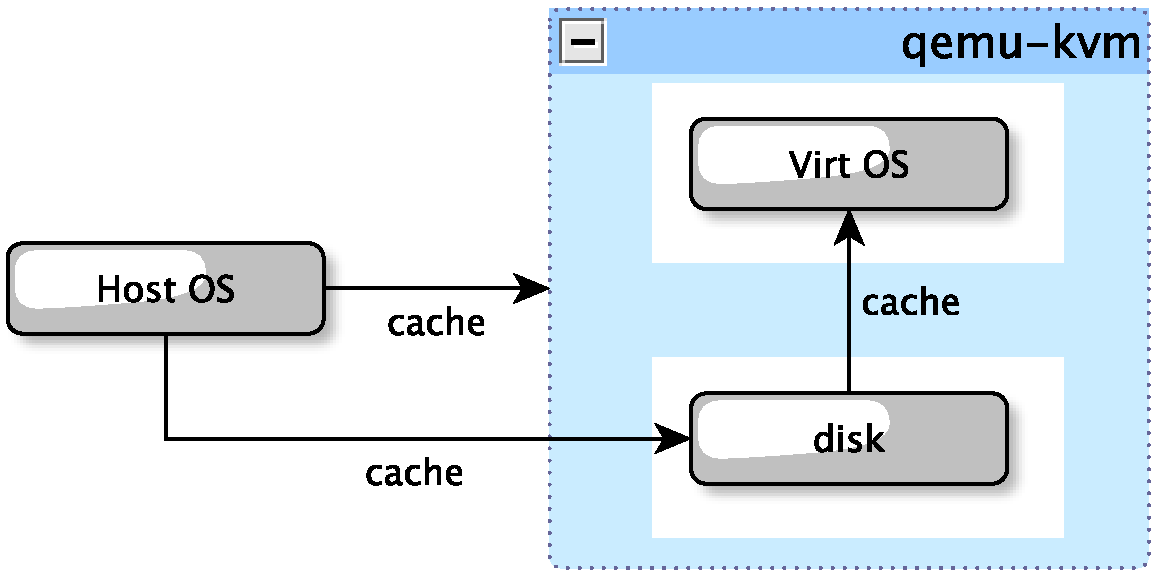
\includegraphics[width=\paperwidth/2]{data/cache.pdf}}
  \caption{Vyznačenie miest, kde môže nastať kešovanie}
  \label{graf-cache}
\end{center}
\end{figure}

Virtualizovaný systém musí obsahovať všetky potrebné balíčky, ktorých programy
sa používajú v~testoch. Ďalej by mali byť vypnuté všetky nepotrebné služby na
pozadí (napríklad \emph{abrtd} alebo \emph{ntp}). Treba si dať pozor aj na
zoznam \emph{cron}\footnote{Časovo závyslí plánovač úloh. Každý užívateľ si
môže naplánovať vykonávanie príkazov v~daných časových intervaloch.} úloh,
ktoré môžeme nájsť v~adresároch \texttt{/etc/cron.*}.

%
% Pouzitie virtualneho stroja
%

\section{Použitie virtuálneho stroja}

Testovanie diskových operácií prebieha vo virtuálnom stroji za použitia
\emph{qemu-kvm} pod \emph{libvirtd}. Tento spôsob testovania som zvolil pre
minimalizáciu problémov, ktoré môžu nastať pri testovaní (popísané v~sekcii
\ref{sec:softverove-rizika}) a~ochránenie hostiteľského operačného systému.

\subsection{Výhody}

Medzi hlavné výhody testovania na virtualizovanom systéme patrí:

\begin{itemize}
    \item Jednoduchšia správa obrazov celého systému.
    \item Pohodlné pripájanie a~odpájanie diskov.
    \item Dokonalé prispôsobenie systému pre požiadavky testov - na
    hostiteľskom systéme moc nezáleží a~dá sa využiť skoro akákoľvek Linuxová
    distribúcia.
\end{itemize}

\subsection{Nevýhody}

Toto testovanie prináša ale aj množstvo nevýhod. 

\begin{itemize}
    \item Hostiteľský systém môže obmedzovať virtualizovaný systém.
    \item Medzi systémami môže nastať kešovanie (ako je zobrazené aj na obrázku
    \ref{graf-cache}). Toto sa ale dá do veľkej miery eliminovať a~nemalo by
    mať vplyv na výsledky testov.
    \item Virtualizovaný systém a~taktiež aj virtuálne disky budú vždy odlišné
    od fyzických. Aj keď virtualízacia beží na úrovni jadra, stále su v
    systémoch malé rozdiely. Preto je celé testovanie experimentálne a~výsledky
    sa budú zbierať a~priemerovať z~viacerých iterácií testovania.
\end{itemize}

\subsection{Zhrnutie}

Aj napriek všetkým nevýhodám je testovanie na virtualizovanom systéme vhodné.
Výsledky testov sú porovnávacie (so zapnutým a~vypnutým \emph{tuned}) - to
znamená, že aj keď by v~skutočnosti časy mohli byť odlišné, rozdiel medzi
\emph{tuned} a~bez \emph{tuned} verziou ostáva rovnaký.

Taktiež treba poznamenať, že je dnes virtualizácia využívaná veľmi často a
preto virtualizácia pri testovaní nie je prekážkou.

%
% Implementacia testov
%

\section{Implementácia testov}

Na implementáciu testov je využitý prevažne jazyk \emph{bash}. Testovanie riadi
hlavný súbor \emph{test\_disk.sh}, v ktorom sa nastavujú parametre testov.
Tieto testy su popísane v tabuľke \ref{tab:test-params}. Konkrétne podtesty
začínajú prefixom \texttt{inc\_*}. Virtuálny systém sa pred každým testom
vypne, obnoví zo zálohy disku a znova zapne.

\begin{table}[H]
\begin{center}
\begin{tabular}{|l|l|}
    \hline
    \textbf{Názov premennej} & \textbf{Popis} \\
    \hline
    TEST\_COMMAND & Sada príkazov pre diskové operácie \\
    FS & Asociatívne pole, obsahujúce názov súborového systému \\ & a príkazu na jeho vytvorenie \\
    TO\_TEST & Zoznam testov, ktoré sa prevedú \\
    \hline
\end{tabular}
\caption{Popis premenných pre parametrizáciu testov.}
\label{tab:test-params}
\end{center}
\end{table}

Disky sa pripájajú podľa toho, ako to vyžaduje aktuálny test. Kešovanie diskov
medzi hostiteľským a virtualizovaným systémom je vypnuté na miestach, ktoré su
uvedené na obrázku \ref{graf-cache}. 

%
% Vyhodnotenie testov
%

\section{Vyhodnotenie testov}

%
% START Automatic results
%
\begin{table}[H]
\begin{center}
\begin{tabular}{|l|r|r|r|}
    \hline
    \textbf{Test} & \textbf{bez tuned} & \textbf{s tuned} & \textbf{rozdiel} \\ \hline
    simple\_disk virtio ext3 & 112 s & 104 s & 8 s \\
    \hline
    raid0 virtio ext3 & 120 s & 111 s & 9 s \\
    \hline
    raid1 virtio ext3 & 131 s & 119 s & 12 s \\
    \hline
\end{tabular}
\caption{Výsledky testov pre súborový systém ext3}
\label{tab:results-ext3}
\end{center}
\end{table}

\begin{table}[H]
\begin{center}
\begin{tabular}{|l|r|r|r|}
    \hline
    \textbf{Test} & \textbf{bez tuned} & \textbf{s tuned} & \textbf{rozdiel} \\ \hline
    simple\_disk virtio ext4 & 116 s & 101 s & 15 s \\
    \hline
    raid0 virtio ext4 & 121 s & 107 s & 14 s \\
    \hline
    raid1 virtio ext4 & 121 s & 109 s & 12 s \\
    \hline
\end{tabular}
\caption{Výsledky testov pre súborový systém ext4}
\label{tab:results-ext4}
\end{center}
\end{table}

%
% END Automatic results
%


%
% Bocné produkty
%

\chapter{Bočné produkty práce}

%
% Libvirt problemy
%

\section{Problém s \emph{libvirtd}}

Pri pripájaní diskov k virtuálnemu systému za použitia príkazu \texttt{virsh
attach-device }, sa systém občas náhodne vypne. Nepodarilo sa mi spoľahlivo
zreprodukovať túto chybu do takého stavu, aby som ju mohol nahlásiť vývojárom,
pretože nastávala nepravidelne. 

O páde systému som nenašiel žiadnu zmienku v logoch virtualizovaného ani
hostovacieho systému. 

%
% Power Management testday
%

\section{Power Management Test Day}

Dňa 17. apríla 2013 sa konal deň otvorených dverí Brnenskej pobočky firmy
\emph{Red Hat}. Súčasťou programu bol aj \emph{Power Management Test Day}
najnovšej verzie operačného systému \emph{Fedora 19}, ktorého som bol
spoluorganizátor. 

Mimo iné sa testovalo aj \emph{tuned} samotné. Najväčším prekvapením bolo
testovanie \emph{tuned} profilu \emph{powersave}, ktorý by mal znižovať
elektrický odber. Na testovanie prišlo množstvo ľudí s rôznymi notebookmi. Konkrétne výsledky sú uvedené v tabuľke \ref{tab:testday-results}.

\begin{table}[H]
\begin{center}
\begin{tabular}{|l|r|r|r|}
    \hline
    \textbf{Typ notebooku} & \textbf{Odber bez tuned} & \textbf{Odber s tuned} \\
    \hline
    Lenovo ThinkPad X230        & 4.540 Wh & 4.110 Wh & 9.47\% \\
    HP Elitebook 8540w          & 7.566 Wh & 7.493 Wh &  \\
    Lenovo T60 laptop           & 4.720 Wh & 4.500 Wh &  \\
    Dell Optiplex 990           & 8.500 Wh & 7.700 Wh &  \\
    Lenovo ThinkPad T61         & 4.880 Wh & 4.340 Wh &  \\
    Lenovo ThinkPad T520        & 5.387 Wh & 4.815 Wh &  \\
    Lenovo T510                 & 3.310 Wh & 2.820 Wh &  \\
    ThinkPad T430               & 5.690 Wh & 5.370 Wh &  \\
    Samsung N210 (Intel Atom)   & 1.402 Wh & 1.394 Wh &  \\
    \hline
\end{tabular}
\caption{Odber rôznych notebookov s vypnutým a zapnutým tuned.}
\label{tab:testday-results}
\end{center}
\end{table}

%
% Najdene chyby
%

\section{Nájdené chyby}

Počas písania tejto bakalárskej práce, narábanie s~\emph{tuned} a~testovaní som
narazil na niekoľko chýb, ktoré som nahlasoval do oficiálnej \emph{Red Hat} a
\emph{Fedora} bugzilly~\cite{rhBugzilla}. Chyby sa nachádzali väčšinou priamo v
balíku \emph{tuned}, ale taktiež v balíku \emph{selinux-policy}.

Tieto chyby boli väčśinou opravené do pár dní. Ich prehľad je v tabuľke \ref{tab:bugs}.

\begin{table}[H]
\begin{center}
\begin{tabular}{|l|l|l|}
    \hline
    \textbf{Číslo chyby} & \textbf{Názov} & \textbf{Status} \\
    \hline
    BZ\#907065 & tuned-adm can crash because of unknown variable log & opravené \\
    BZ\#953128 & tuned does not start if active profile is missing & opravené \\
    BZ\#953132 & AVCs after starting tuned daemon & opravené \\
    BZ\#901689 & Typo in tuned-adm.py & opravené \\
    BZ\#911138 & tuned-adm profile virtual-guest/host AVC denied & zatiaľ neopravené \\
    \hline
\end{tabular}
\caption{Zoznam nájdených chýb}
\label{tab:bugs}
\end{center}
\end{table}


%
% Zaver 
%

\chapter{Záver}

Z výsledkov je jasné, že \emph{tuned} naozaj optimalizuje I/O operácie na
diskových poliach. 
